% Created by tikzDevice version 0.12.3.1 on 2021-12-15 13:57:49
% !TEX encoding = UTF-8 Unicode
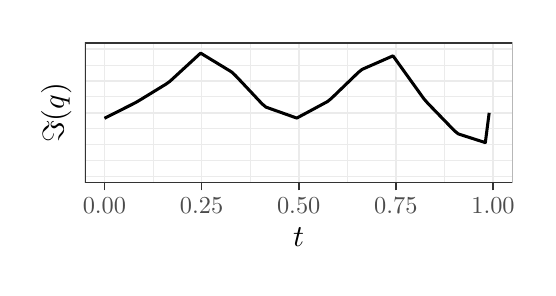
\begin{tikzpicture}[x=1pt,y=1pt]
\definecolor{fillColor}{RGB}{255,255,255}
\path[use as bounding box,fill=fillColor,fill opacity=0.00] (0,0) rectangle (180.67, 86.72);
\begin{scope}
\path[clip] (  0.00,  0.00) rectangle (180.67, 86.72);
\definecolor{drawColor}{RGB}{255,255,255}
\definecolor{fillColor}{RGB}{255,255,255}

\path[draw=drawColor,line width= 0.6pt,line join=round,line cap=round,fill=fillColor] (  0.00,  0.00) rectangle (180.67, 86.72);
\end{scope}
\begin{scope}
\path[clip] ( 20.71, 30.69) rectangle (175.17, 81.22);
\definecolor{fillColor}{RGB}{255,255,255}

\path[fill=fillColor] ( 20.71, 30.69) rectangle (175.17, 81.22);
\definecolor{drawColor}{gray}{0.92}

\path[draw=drawColor,line width= 0.3pt,line join=round] ( 20.71, 38.73) --
	(175.17, 38.73);

\path[draw=drawColor,line width= 0.3pt,line join=round] ( 20.71, 50.21) --
	(175.17, 50.21);

\path[draw=drawColor,line width= 0.3pt,line join=round] ( 20.71, 61.70) --
	(175.17, 61.70);

\path[draw=drawColor,line width= 0.3pt,line join=round] ( 20.71, 73.18) --
	(175.17, 73.18);

\path[draw=drawColor,line width= 0.3pt,line join=round] ( 45.29, 30.69) --
	( 45.29, 81.22);

\path[draw=drawColor,line width= 0.3pt,line join=round] ( 80.39, 30.69) --
	( 80.39, 81.22);

\path[draw=drawColor,line width= 0.3pt,line join=round] (115.50, 30.69) --
	(115.50, 81.22);

\path[draw=drawColor,line width= 0.3pt,line join=round] (150.60, 30.69) --
	(150.60, 81.22);

\path[draw=drawColor,line width= 0.6pt,line join=round] ( 20.71, 32.98) --
	(175.17, 32.98);

\path[draw=drawColor,line width= 0.6pt,line join=round] ( 20.71, 44.47) --
	(175.17, 44.47);

\path[draw=drawColor,line width= 0.6pt,line join=round] ( 20.71, 55.95) --
	(175.17, 55.95);

\path[draw=drawColor,line width= 0.6pt,line join=round] ( 20.71, 67.44) --
	(175.17, 67.44);

\path[draw=drawColor,line width= 0.6pt,line join=round] ( 20.71, 78.93) --
	(175.17, 78.93);

\path[draw=drawColor,line width= 0.6pt,line join=round] ( 27.74, 30.69) --
	( 27.74, 81.22);

\path[draw=drawColor,line width= 0.6pt,line join=round] ( 62.84, 30.69) --
	( 62.84, 81.22);

\path[draw=drawColor,line width= 0.6pt,line join=round] ( 97.94, 30.69) --
	( 97.94, 81.22);

\path[draw=drawColor,line width= 0.6pt,line join=round] (133.05, 30.69) --
	(133.05, 81.22);

\path[draw=drawColor,line width= 0.6pt,line join=round] (168.15, 30.69) --
	(168.15, 81.22);
\definecolor{drawColor}{RGB}{0,0,0}

\path[draw=drawColor,line width= 1.1pt,line join=round] ( 27.74, 53.96) --
	( 29.13, 54.66) --
	( 30.52, 55.36) --
	( 31.91, 56.06) --
	( 33.30, 56.76) --
	( 34.69, 57.47) --
	( 36.08, 58.17) --
	( 37.47, 58.87) --
	( 38.86, 59.57) --
	( 40.25, 60.37) --
	( 41.64, 61.22) --
	( 43.03, 62.07) --
	( 44.42, 62.92) --
	( 45.81, 63.77) --
	( 47.20, 64.62) --
	( 48.59, 65.47) --
	( 49.98, 66.32) --
	( 51.37, 67.31) --
	( 52.76, 68.58) --
	( 54.15, 69.86) --
	( 55.54, 71.14) --
	( 56.93, 72.41) --
	( 58.32, 73.69) --
	( 59.71, 74.97) --
	( 61.10, 76.25) --
	( 62.49, 77.52) --
	( 63.88, 76.68) --
	( 65.27, 75.83) --
	( 66.66, 74.99) --
	( 68.05, 74.15) --
	( 69.44, 73.30) --
	( 70.83, 72.46) --
	( 72.22, 71.61) --
	( 73.61, 70.77) --
	( 75.00, 69.50) --
	( 76.40, 68.02) --
	( 77.79, 66.55) --
	( 79.18, 65.07) --
	( 80.57, 63.59) --
	( 81.96, 62.11) --
	( 83.35, 60.63) --
	( 84.74, 59.15) --
	( 86.13, 58.00) --
	( 87.52, 57.51) --
	( 88.91, 57.01) --
	( 90.30, 56.52) --
	( 91.69, 56.03) --
	( 93.08, 55.53) --
	( 94.47, 55.04) --
	( 95.86, 54.54) --
	( 97.25, 54.05) --
	( 98.64, 54.80) --
	(100.03, 55.54) --
	(101.42, 56.29) --
	(102.81, 57.04) --
	(104.20, 57.79) --
	(105.59, 58.54) --
	(106.98, 59.29) --
	(108.37, 60.04) --
	(109.76, 61.18) --
	(111.15, 62.52) --
	(112.54, 63.86) --
	(113.93, 65.20) --
	(115.32, 66.54) --
	(116.71, 67.88) --
	(118.10, 69.22) --
	(119.49, 70.57) --
	(120.88, 71.66) --
	(122.27, 72.27) --
	(123.66, 72.88) --
	(125.06, 73.49) --
	(126.45, 74.10) --
	(127.84, 74.71) --
	(129.23, 75.32) --
	(130.62, 75.93) --
	(132.01, 76.54) --
	(133.40, 74.61) --
	(134.79, 72.67) --
	(136.18, 70.74) --
	(137.57, 68.80) --
	(138.96, 66.87) --
	(140.35, 64.94) --
	(141.74, 63.00) --
	(143.13, 61.07) --
	(144.52, 59.47) --
	(145.91, 58.03) --
	(147.30, 56.60) --
	(148.69, 55.16) --
	(150.08, 53.73) --
	(151.47, 52.29) --
	(152.86, 50.86) --
	(154.25, 49.42) --
	(155.64, 48.32) --
	(157.03, 47.87) --
	(158.42, 47.42) --
	(159.81, 46.98) --
	(161.20, 46.53) --
	(162.59, 46.08) --
	(163.98, 45.64) --
	(165.37, 45.19) --
	(166.76, 55.95);
\definecolor{drawColor}{gray}{0.20}

\path[draw=drawColor,line width= 0.6pt,line join=round,line cap=round] ( 20.71, 30.69) rectangle (175.17, 81.22);
\end{scope}
\begin{scope}
\path[clip] (  0.00,  0.00) rectangle (180.67, 86.72);
\definecolor{drawColor}{gray}{0.20}

\path[draw=drawColor,line width= 0.6pt,line join=round] ( 27.74, 27.94) --
	( 27.74, 30.69);

\path[draw=drawColor,line width= 0.6pt,line join=round] ( 62.84, 27.94) --
	( 62.84, 30.69);

\path[draw=drawColor,line width= 0.6pt,line join=round] ( 97.94, 27.94) --
	( 97.94, 30.69);

\path[draw=drawColor,line width= 0.6pt,line join=round] (133.05, 27.94) --
	(133.05, 30.69);

\path[draw=drawColor,line width= 0.6pt,line join=round] (168.15, 27.94) --
	(168.15, 30.69);
\end{scope}
\begin{scope}
\path[clip] (  0.00,  0.00) rectangle (180.67, 86.72);
\definecolor{drawColor}{gray}{0.30}

\node[text=drawColor,anchor=base,inner sep=0pt, outer sep=0pt, scale=  0.88] at ( 27.74, 19.68) {0.00};

\node[text=drawColor,anchor=base,inner sep=0pt, outer sep=0pt, scale=  0.88] at ( 62.84, 19.68) {0.25};

\node[text=drawColor,anchor=base,inner sep=0pt, outer sep=0pt, scale=  0.88] at ( 97.94, 19.68) {0.50};

\node[text=drawColor,anchor=base,inner sep=0pt, outer sep=0pt, scale=  0.88] at (133.05, 19.68) {0.75};

\node[text=drawColor,anchor=base,inner sep=0pt, outer sep=0pt, scale=  0.88] at (168.15, 19.68) {1.00};
\end{scope}
\begin{scope}
\path[clip] (  0.00,  0.00) rectangle (180.67, 86.72);
\definecolor{drawColor}{RGB}{0,0,0}

\node[text=drawColor,anchor=base,inner sep=0pt, outer sep=0pt, scale=  1.10] at ( 97.94,  7.64) {$t$};
\end{scope}
\begin{scope}
\path[clip] (  0.00,  0.00) rectangle (180.67, 86.72);
\definecolor{drawColor}{RGB}{0,0,0}

\node[text=drawColor,rotate= 90.00,anchor=base,inner sep=0pt, outer sep=0pt, scale=  1.10] at ( 13.08, 55.95) {$\Im(q)$};
\end{scope}
\end{tikzpicture}
